\subsection{From Pipeline to Design Space}
\label{subsec:design_space}

\newcommand{\compacteq}[1]{%
{\setlength{\abovedisplayskip}{3pt}%
\setlength{\belowdisplayskip}{3pt}%
\setlength{\abovedisplayshortskip}{1pt}%
\setlength{\belowdisplayshortskip}{1pt}%
\[
#1
\]}}

% \begin{figure*}[ht]
%     \centering
%     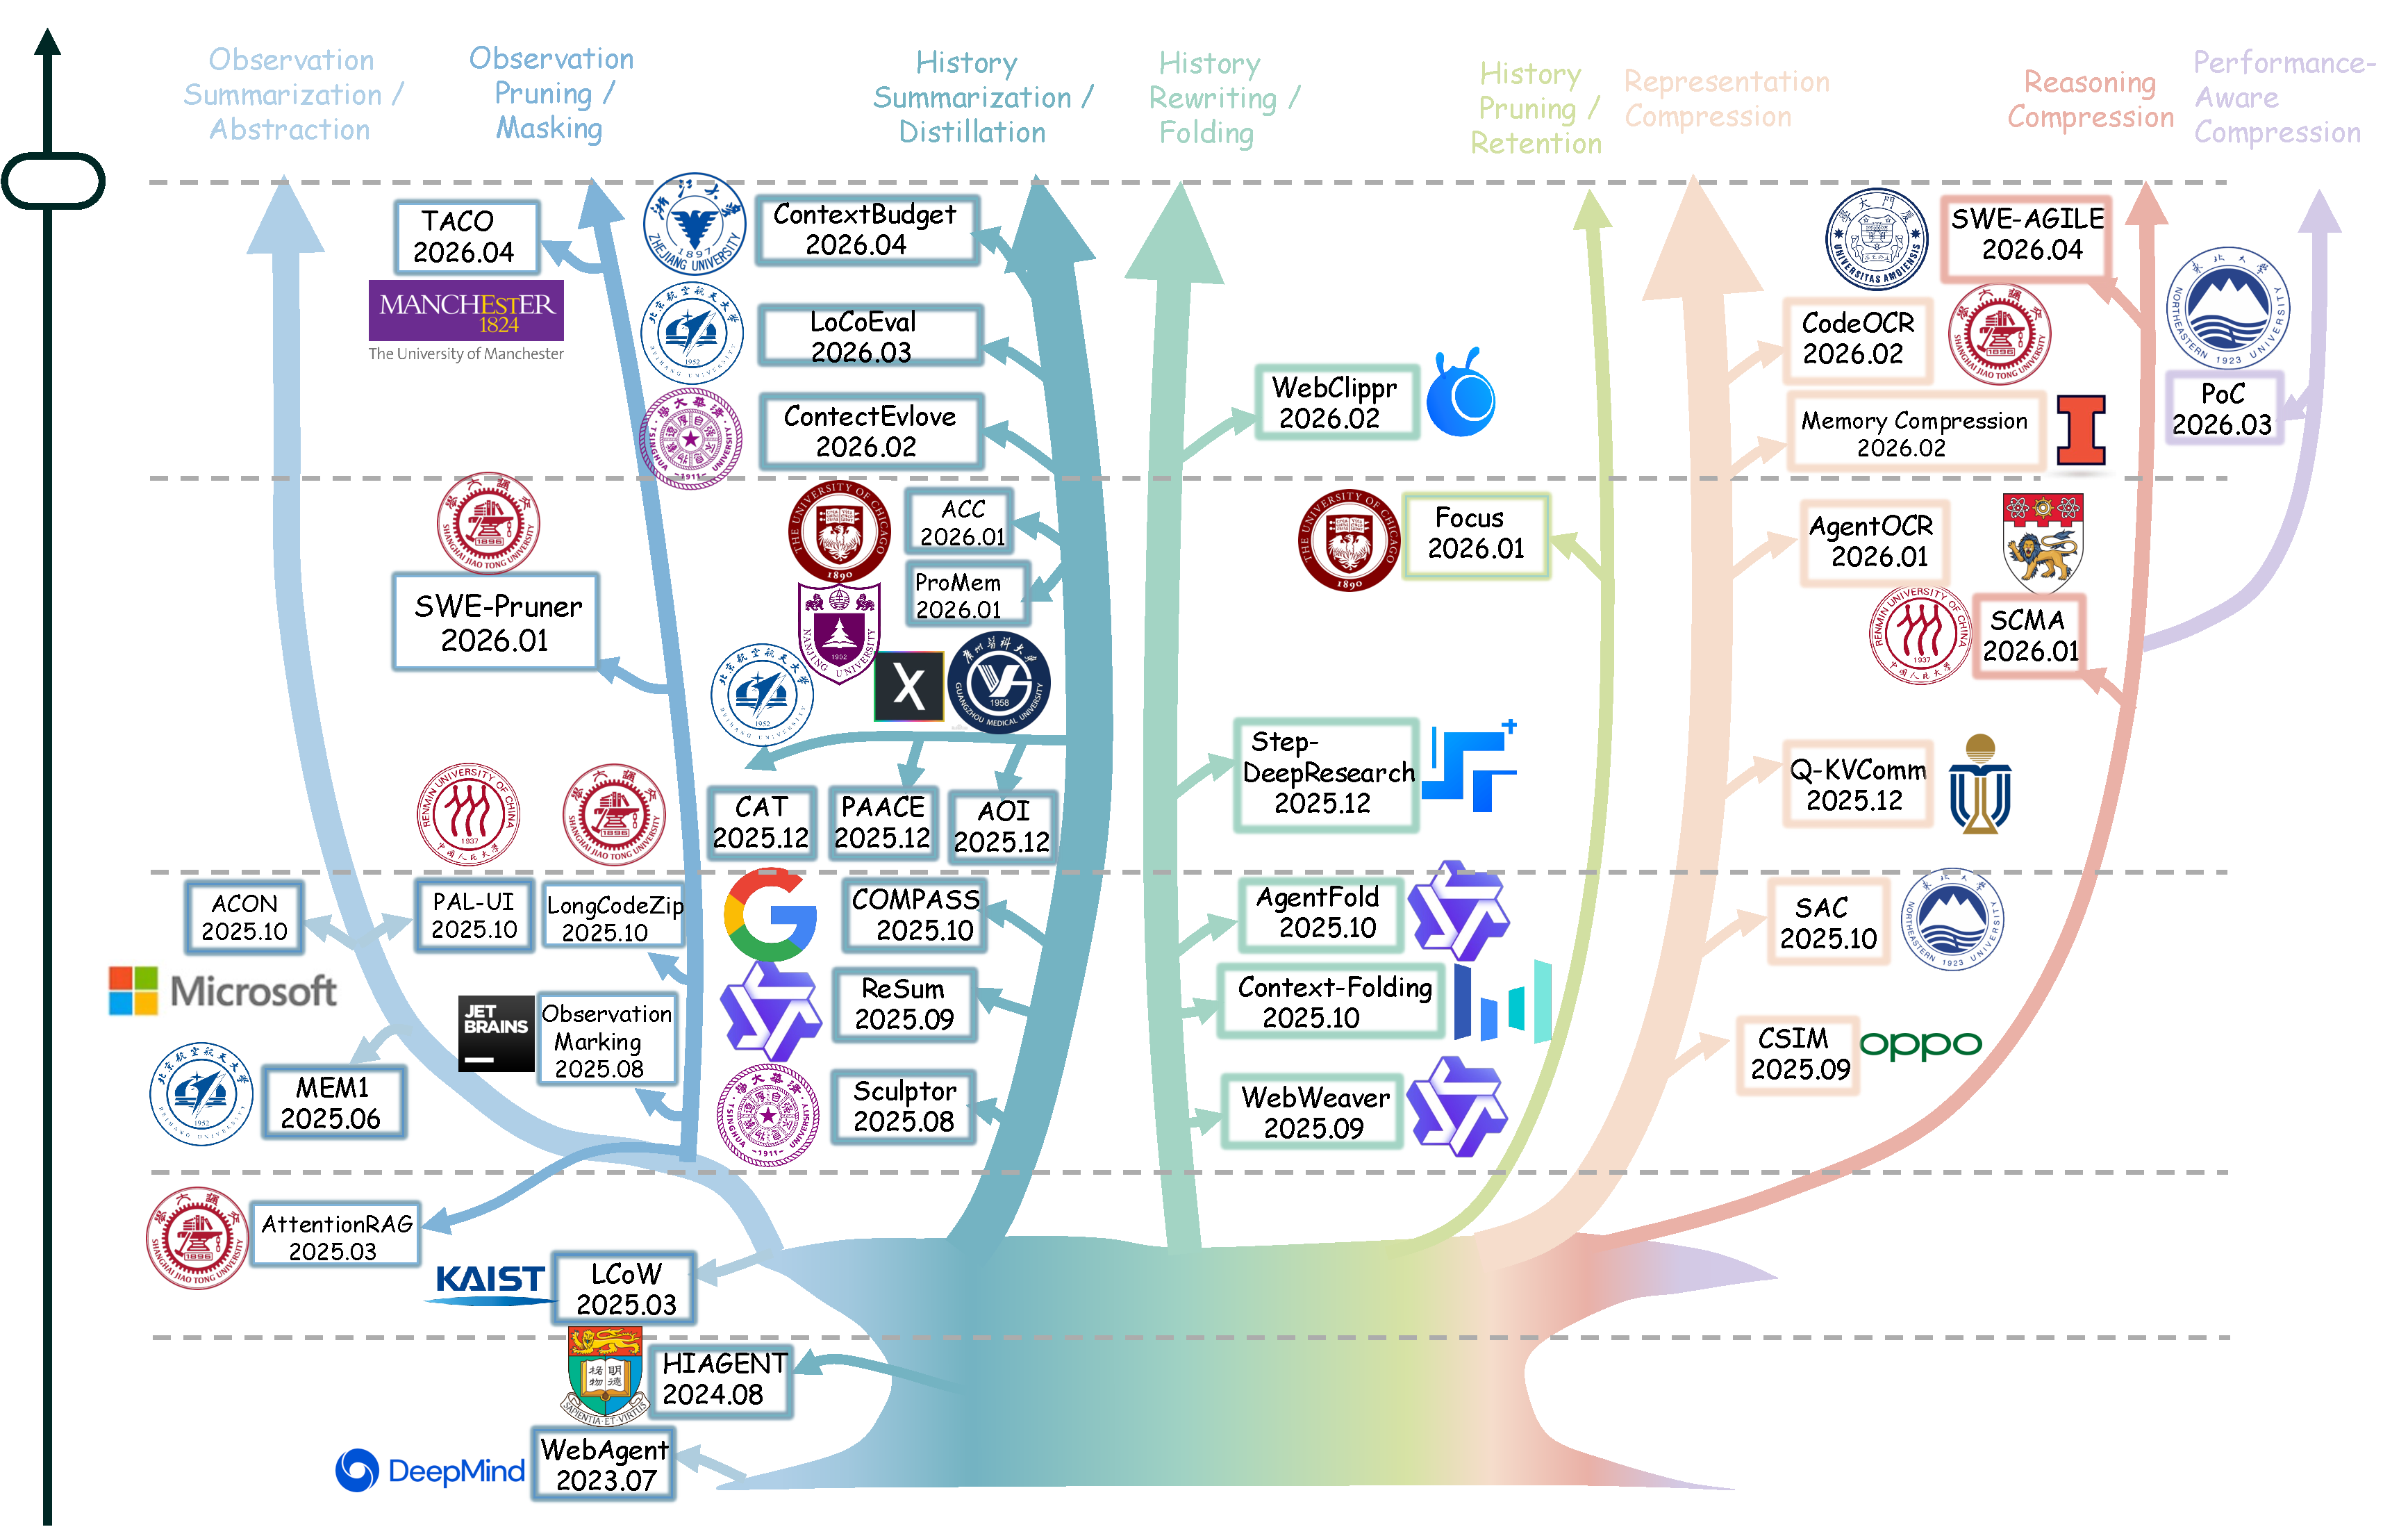
\includegraphics[width=0.74\textwidth]{figures/taxonomy.pdf}
%     \vspace{-.2cm}
%     \caption{A design-space view of agent context compression. The figure synthesizes targets, mechanisms, and control policies into a method-level landscape, grouping approaches by compression semantics while preserving chronological evolution.}
%     \label{fig:taxonomy_tree}
% \end{figure*}


The unified pipeline in \S~\ref{subsec:unified_pipeline} can be read as a comparative design space for agent compression. We organize the literature along three axes: \textit{what} is selected for compression, \textit{how} it is transformed, and \textit{who} decides when compression occurs. These axes map naturally onto the pipeline: targets define the input to \textbf{Select} ($S$), mechanisms implement \textbf{Compress} ($\Phi$) and \textbf{Store} ($M$), and control policies govern when these stages, and when necessary \textbf{Recover} ($R$), are invoked.
\vspace{0.8em}

\begin{table*}[t]
\centering
\small
\begin{tabular}{@{}p{2.4cm}p{2.6cm}p{1.5cm}p{1.5cm}p{1.8cm}p{3.5cm}@{}}
\toprule
\textbf{\raisebox{-0.15em}{
\includegraphics[height=1em]{icons/target.pdf}}~Target} & \textbf{\raisebox{-0.15em}{
\includegraphics[height=1em]{icons/pyramid.pdf}}~Granularity} & \textbf{Information Density} & \textbf{Causal Coupling} & \textbf{Recoverability} & \textbf{\raisebox{-0.15em}{
\includegraphics[height=1em]{icons/failure.pdf}}~Typical Failure Symptom} \\
\midrule
\textbf{Observation} & Token / Segment & Very Low & Weak & Low & Structural Distortion \\
\textbf{Trajectory} & Episode & Low & Moderate & Moderate & Planning Drift \\
\textbf{Plan \& Reasoning} & State & High & Very Strong & Very Low & Metacognitive Error \\
\textbf{Memory State} & State & High & Strong & Very Low & Retrieval Blindness \\
\textbf{Representation} & Token / Latent & Very High & None & None & Semantic Collapse \\
\bottomrule
\end{tabular}
% \vspace{-.2cm}
\caption{A comparative anatomy of compression targets. Each target is characterized by its granularity, information density, causal coupling, and recoverability, which collectively shape its compressibility and its failure symptom.}
\label{tab:target_comparison}
\vspace{-.2in}
\end{table*}

\subsection{Compression Targets (\textit{What})}
\label{subsec:compressin_target}

We begin with the objects processed by the \textbf{Select} ($S$) operator. Table~\ref{tab:target_comparison} summarizes these targets in terms of granularity, information density, causal coupling, and recoverability. Together, these properties determine both compressibility and likely failure symptoms.

\subsubsection{Observation Compression}
Observation compression targets raw inputs, such as tool outputs, HTML DOMs, logs, or screenshots. These inputs are high-volume and redundant, but a single omitted selector, trace line, or visual cue may determine the next action. Methods such as The Complexity Trap~\citep{lindenbauer2025complexitytrapsimpleobservation} therefore treat it as a low-cost front-end intervention, typically via masking or shallow filtering.

\subsubsection{Trajectory Compression}
Trajectory compression focuses on accumulated multi-step histories, including failed attempts, redundant tool calls, and repetitive loops. Its main difficulty is deferred utility: information that appears irrelevant at step $t$ may become indispensable later. As a result, trajectory compression is especially vulnerable to \ftwo \quad and delayed downstream inconsistency. Representative approaches include controller-mediated reduction in AgentDiet~\citep{xiao2025improving}, periodic summarization in ReSum~\citep{wu2026resumunlockinglonghorizonsearch}, and proactive folding in AgentFold~\citep{ye2025agentfoldlonghorizonwebagents}.

\subsubsection{Plan and Reasoning Compression}
Plan and reasoning compression targets internal artifacts, including subgoals, deliberative traces, self-reflections, and task decompositions. These representations are compact but brittle: dropping a seemingly minor premise can invalidate an entire downstream plan. This target is therefore  sensitive to \fone, because the system must correctly judge which reasoning artifacts remain decision-critical. Representative methods include feedback-driven summarization in ACON~\citep{kang2025aconoptimizingcontextcompression} and agent-initiated memory management in Focus~\citep{verma2026activecontextcompressionautonomous}.


\subsubsection{Memory State Compression}
Memory state compression maps an unbounded interaction stream into a fixed-capacity representation that survives beyond the immediate context window. It most explicitly realizes the \textbf{Store} ($M$) stage, so its main bottleneck is accessibility rather than faithfulness. Once information is offloaded, the system must still recognize when that memory matters and reconstruct it at use time. Consequently, memory-state compression is most directly exposed to \fthree. Learned memory policies such as MEM1~\citep{zhou2025mem1learningsynergizememory} address this challenge by coupling state formation with future retrieval utility.

\subsubsection{Representation-Level Compression}
Representation-level compression operates below the natural-language interface, targeting KV caches, multimodal token embeddings, or other latent states. It often delivers the strongest efficiency gains, but with minimal recoverability and weak inspectability. These methods therefore shift the problem from semantic editing to opaque state management. Representative examples include AgentOCR~\citep{feng2026agentocrreimaginingagenthistory}, Q-KVComm~\citep{kriuk2025qkvcommefficientmultiagentcommunication}, and SAC~\citep{liu2026autoencodingfreecontextcompressionllms}.


\subsection{Compression Mechanisms (\textit{How})}
\label{subsec:compression_mechanism}

% Having identified the targets, we now turn to the transformations themselves. Mechanisms differ in the relation they preserve between the compressed artifact and the source context: some delete spans outright, some rewrite them semantically, some retain only an exact subset, and others offload information into an explicitly recoverable store. This distinction is central because methods with similar compression ratios can differ sharply in faithfulness, inspectability, and downstream recoverability.
Having identified the targets, we now turn to the transformations themselves. What most distinguishes compression mechanisms is how they relate the compressed result to the original context. Some remove content, some paraphrase it, some retain an exact subset, and others store information so that it can be recovered later. This distinction is crucial because methods with similar compression ratios may differ sharply in \emph{faithfulness}, \emph{inspectability}, and \emph{downstream recoverability}.

\subsubsection{Masking and Truncation} 
These operators keep a prefix or suffix of the context, or selectively mask designated spans:
\compacteq{O_{\mathrm{trunc}}(\mathcal{C}) = \mathcal{C}[:k],\; O_{\mathrm{mask}}(\mathcal{C}) = \mathrm{mask}(\mathcal{C}, S).}
These operators, which directly modify the support of \(C\) through span removal or placeholder substitution, are universal, low-overhead, and easy to deploy. That same directness also defines their limitation: once content is removed, recoverability is lost unless another subsystem stores it elsewhere. Such operators are therefore best suited to settings in which marginal utility decays rapidly with recency or position, as in sliding-window baselines or hard budget enforcement~\citep{wang2025mcpbenchbenchmarkingtoolusingllm}.

\subsubsection{Summarization and Abstraction} 
These operators rewrite a long context into a shorter semantic representation:
\compacteq{O_{\mathrm{sum}}(\mathcal{C}) = \hat{C},\; |\hat{C}| \ll |\mathcal{C}|.}
Unlike truncation, summarization preserves utility by semantic rewriting rather than direct deletion. This often yields substantially higher information density and better long-horizon compactness, which explains its popularity in research and search agents. The trade-off is that faithfulness becomes model-dependent: once context is rewritten, omissions, over-generalizations, and spurious inferences may be introduced, making summarization a primary locus of \ftwo. Representative systems include LCoW~\citep{lee2025learningcontextualizewebpages}, COMPASS~\citep{wan2025compassenhancingagentlonghorizon}, and ReSum~\citep{wu2026resumunlockinglonghorizonsearch}.


% \subsubsection{Masking and Truncation} 
% These operators keep a prefix or suffix of the context, or selectively mask designated spans:
% \compacteq{O_{\mathrm{trunc}}(\mathcal{C}) = \mathcal{C}[:k],\; O_{\mathrm{mask}}(\mathcal{C}) = \mathrm{mask}(\mathcal{C}, S).}
% They directly modify the support of \(C\) through span removal or placeholder substitution. Their appeal lies in universality, low overhead, and ease of deployment. Their limitation is equally direct: once content is removed, recoverability is lost unless another subsystem stores it elsewhere. These operators are therefore best suited to settings in which marginal utility decays rapidly with recency or position, as in sliding-window baselines or hard budget enforcement~\citep{wang2025mcpbenchbenchmarkingtoolusingllm}.

% \subsubsection{Summarization and Abstraction} 
% These operators rewrite a long context into a shorter semantic representation:
% \compacteq{O_{\mathrm{sum}}(\mathcal{C}) = \hat{C},\; |\hat{C}| \ll |\mathcal{C}|.}
% Unlike truncation, they preserve utility by semantic rewriting rather than direct deletion. This often yields substantially higher information density and better long-horizon compactness, which explains their popularity in research and search agents. The trade-off is that faithfulness becomes model-dependent: once context is rewritten, omissions, over-generalizations, and spurious inferences may be introduced, making summarization a primary locus of \ftwo. Representative systems include LCoW~\citep{lee2025learningcontextualizewebpages}, COMPASS~\citep{wan2025compassenhancingagentlonghorizon}, and ReSum~\citep{wu2026resumunlockinglonghorizonsearch}.

\subsubsection{Pruning and Reduction} 
Pruning removes content selectively while preserving the remaining structure exactly:
\compacteq{O_{\mathrm{prune}}(\mathcal{C}) = \mathcal{C} \setminus R,}
where \(R\) is a subset selected by a relevance, dependency, or structural criterion. Unlike summarization, pruning leaves retained evidence untouched. It is therefore especially valuable when syntactic form, pointer alignment, or execution traces must remain exact, as in coding and GUI settings. In exchange, pruning typically compresses less aggressively than summarization unless the context contains substantial redundancy. Representative examples include SWE-Pruner~\citep{wang2026sweprunerselfadaptivecontextpruning} and WebClipper~\citep{wang2026webclipperefficientevolutionweb}.

\subsubsection{Externalization and Retrieval} 
This mechanism splits context into a working state and an external store:
\compacteq{O_{\mathrm{ext}}(\mathcal{C}) = (C', M),\; O_{\mathrm{ret}}(\mathcal{C}, M) = \mathcal{C} \oplus r(M).}
It is the clearest realization of \textbf{Store} ($M$) and \textbf{Recover} ($R$) in the pipeline. By turning part of compression into retrieval, it permits aggressive footprint reduction so long as critical information can later be reconstructed on demand. It is therefore the only mechanism that combines high compression with principled recoverability. Its main risk shifts toward \fthree: not corruption, but missing, mistimed, or incorrect re-access. Systems such as Step-DeepResearch~\citep{hu2025stepdeepresearchtechnicalreport}, CAT~\citep{liu2025contexttoolcontextmanagement}, and WebWeaver~\citep{li2025webweaverstructuringwebscaleevidence} rely heavily on this paradigm.

% \subsubsection{Externalization and Retrieval} 
% This mechanism splits context into a working state and an external store:
% \compacteq{O_{\mathrm{ext}}(\mathcal{C}) = (C', M),\; O_{\mathrm{ret}}(\mathcal{C}, M) = \mathcal{C} \oplus r(M).}
% It is the clearest realization of \textbf{Store} ($M$) and \textbf{Recover} ($R$) in the pipeline. Conceptually, it converts part of the compression problem into a retrieval problem: instead of forcing all useful information to remain in the active context, it permits aggressive footprint reduction so long as critical information can later be reconstructed on demand. This makes it the only mechanism that simultaneously supports high compression and principled recoverability. Its failure mode is correspondingly shifted toward \fthree, because the main risk is no longer only information corruption but missing, mistimed, or incorrect re-access. Systems such as Step-DeepResearch~\citep{hu2025stepdeepresearchtechnicalreport}, CAT~\citep{liu2025contexttoolcontextmanagement}, and WebWeaver~\citep{li2025webweaverstructuringwebscaleevidence} rely heavily on this paradigm.
% \begin{figure*}[t]
%     \centering
%     \captionbox{A temporal taxonomy of context compression failures. Failures are classified by the earliest point at which they occur in the compression pipeline.\label{fig:failure_modes_taxonomy}}[0.48\textwidth]{%
%     \makebox[\linewidth][l]{%
%         \raisebox{-0.3mm}[0pt][0pt]{%
%             \scalebox{1}[1.1]{%
%                 
\includegraphics[width=\linewidth]{figures/section5.pdf}%
%             }%
%         }%
%     }%
%     \vspace{-.2cm}
% }
%     \hfill
%     \captionbox{Domain-specific context compression regimes, contrasting setup, workflow, interaction loop, dominant risks, and strategy choices.\label{fig:domain_specific_regimes}}[0.49\textwidth]{%
%         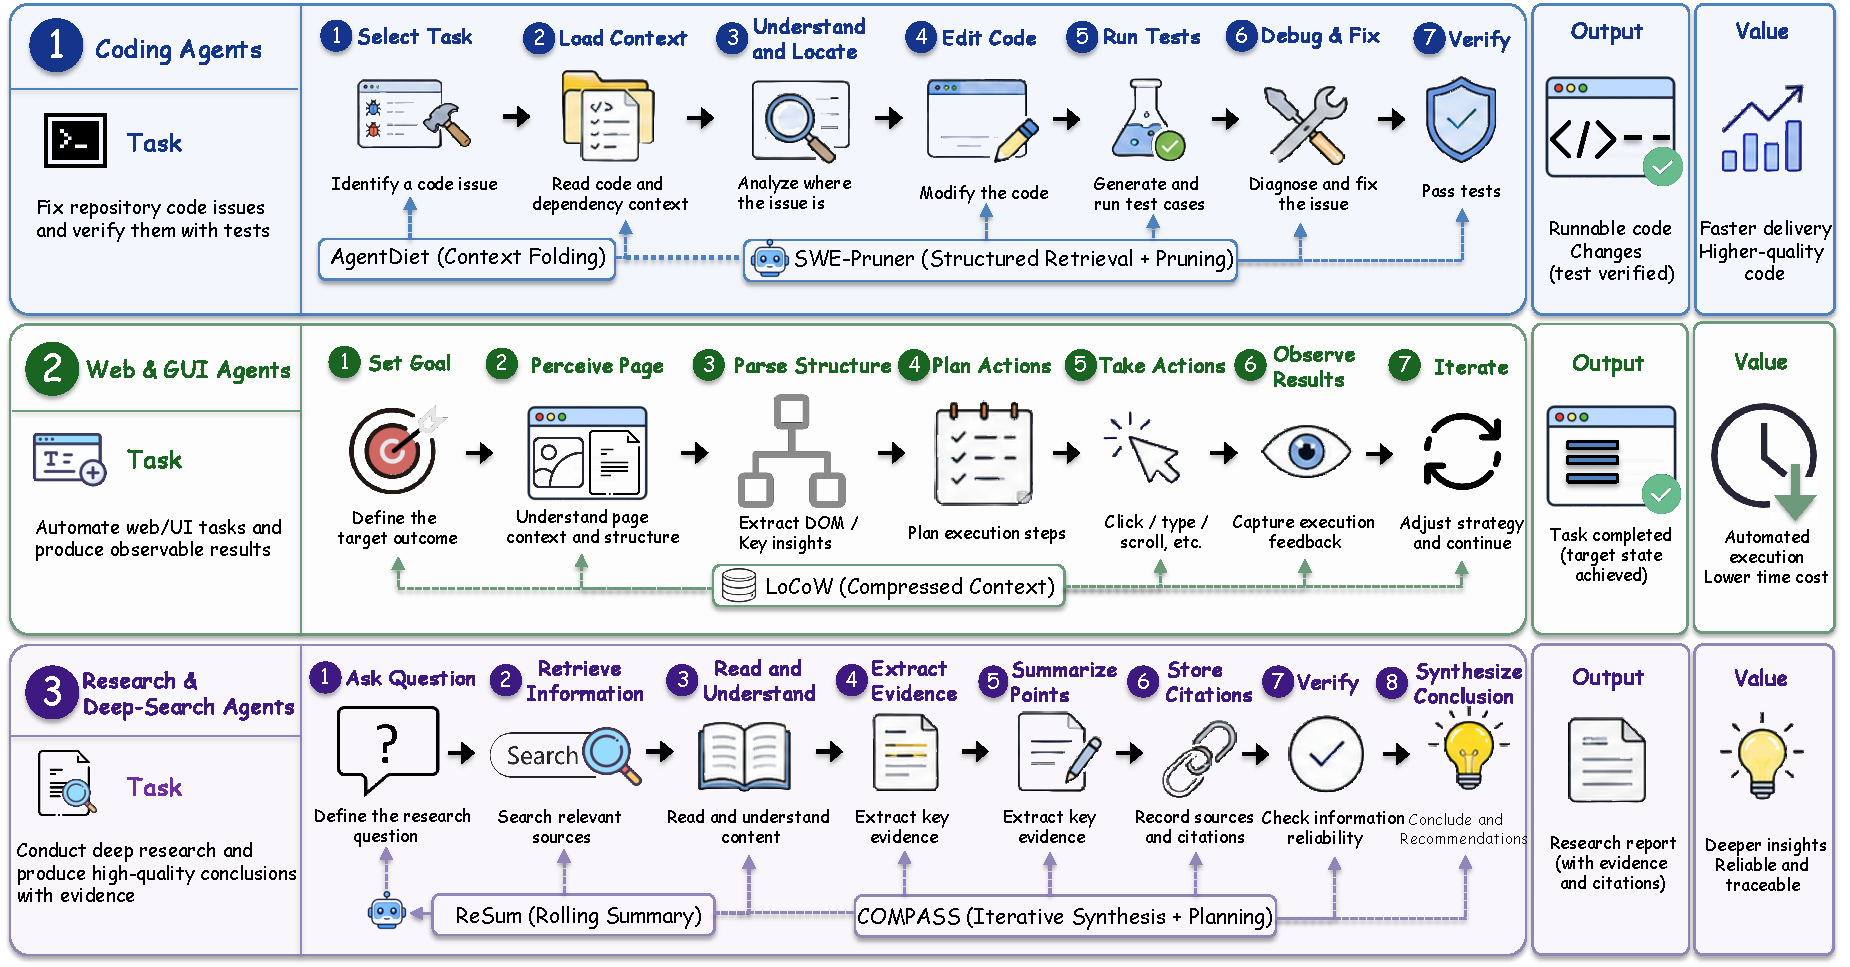
\includegraphics[width=.85\linewidth]{figures/section6.pdf}
%         \vspace{-.2cm}
%     }
% \vspace{-.3cm}
% \end{figure*}

\subsubsection{Representation Compression} 
Operating on latent structures, \(O_{\mathrm{repr}}(\mathcal{C}) = \tilde{C}\) compresses history without explicit textual rewriting. These methods optimize efficiency most directly, but they do so by moving compression beneath the symbolic interface available to the agent and the researcher. As a result, they offer limited interpretability, weak controllability, and little explicit support for exact recovery. Methods such as DebateOCR~\citep{wu2026crossmodalmemorycompressionefficient} illustrate this trade-off.


\subsection{Control Policies and Intervention Timing (\textit{Who} and \textit{When})}
\label{subsec:compression_policy}

Control policy, not compression mechanism, determines when intervention occurs. The same operator may be triggered reactively at a budget threshold, periodically by an external controller, or proactively by the agent itself. We therefore separate operator family from control policy: policy specifies when \textbf{Select}, \textbf{Compress}, and, where applicable, \textbf{Recover} are invoked, who makes that decision, and which signals are sufficient to trigger action.


\subsubsection{System-Controlled Policies} 
System-controlled policies apply fixed rules to trigger compression:
\compacteq{\pi_{\mathrm{sys}} : \mathcal{C} \mapsto (i, \theta).}
Depending only on observable signals such as length, position, or step count, they are predictable, cheap, and easy to benchmark. Their weakness is semantic blindness: they intervene because a budget is reached, not because task utility has changed. Such policies therefore dominate early and production-constrained systems, including predefined schedules in AgentDiet~\citep{xiao2025improving} and threshold-based compaction regimes.

\subsubsection{External Controller Policies} 
External-controller policies delegate the decision to a separate module:
\compacteq{\pi_{\mathrm{ext}} : \mathcal{C} \rightarrow (i, \theta).}
The controller may be a smaller model, a planner, or a retrieval manager that observes the evolving context and selects a compression action for the main agent. This decoupling improves modularity and sometimes yields more stable control, because compression can be optimized independently of task execution. The cost is additional latency, token overhead, and a new interface on which information can be lost. Examples include PAL-UI~\citep{liu2025paluiplanningactivelookback} and AOI~\citep{bai2026aoicontextawaremultiagentoperations}.

\subsubsection{Agent-Controlled Policies} 
Agent-controlled policies make compression part of the agent's own action space:
\compacteq{\pi_{\mathrm{agent}}(C_t, s_t) \rightarrow (i, \theta),}
where \(s_t\) denotes the agent's internal state. This policy class is the most semantically aware, because the same system that reasons about the task also decides which context should be compressed, preserved, or revisited. It is therefore well suited to proactive memory management and self-reflective intervention, as in CAT~\citep{liu2025contexttoolcontextmanagement}, Focus~\citep{verma2026activecontextcompressionautonomous}, and ContextBudget~\citep{wu2026contextbudgetbudgetawarecontextmanagement}. Its weakness is precisely the agent's own fallibility: errors in self-assessment readily manifest as \fone.

\subsubsection{Learned Compression Policies} 
Learned policies optimize compression behavior from data:
\compacteq{\pi_{\mathrm{learn}} = \arg\max_{\pi} \mathbb{E}_{\tau \sim \pi} \left[ R_{\mathrm{task}}(\tau) - \lambda \, \mathrm{Cost}(\tau) \right].}
Whether trained by supervised fine-tuning or reinforcement learning, they seek to align compression decisions with downstream task return rather than handcrafted heuristics. This makes them the most expressive policy class and, in principle, the closest approximation to the ideal sufficient-memory objective in Section~\ref{sec:3_formal_view}. In practice, however, they are also the most resource-intensive and the most sensitive to reward misspecification. Representative examples include ACON~\citep{kang2025aconoptimizingcontextcompression}, MEM1~\citep{zhou2025mem1learningsynergizememory}, and related policy-learning approaches.
